\section[\englishfont 1 研究背景]{研究背景}
\subsection[\englishfont 1.1 车联网]{1.1 车联网}

\begin{frame}{智能交通系统驱动核心}
\frametitle{\englishfont 智能交通系统驱动核心}
\newBackground
\begin{center}
\begin{textblock*}{\textwidth}(1cm,2cm)
\begin{spacing}{0}
  \small \colorbox{cqublue}{\color{white}{车联网及其所驱动的}}
\end{spacing}
\end{textblock*}
\end{center}

\begin{center}
\begin{textblock*}{\textwidth}(1cm,2.5cm)
\begin{spacing}{0}
  \small \colorbox{cqublue}{\color{white}{智能交通与智慧城市}}
\end{spacing}
\end{textblock*}
\end{center}

\begin{center}
\begin{textblock*}{\textwidth}(1cm,6.5cm)
\begin{spacing}{0}
  \small \colorbox{cqublue}{\color{white}{推动汽车向}\color{yellow}{网联化、智}}
\end{spacing}
\end{textblock*}
\end{center}

\begin{center}
\begin{textblock*}{\textwidth}(1cm,7cm)
\begin{spacing}{0}
  \small \colorbox{cqublue}{\color{yellow}{能化与协同化}\color{white}{方向演进}}
\end{spacing}
\end{textblock*}
\end{center}

\begin{center}
\begin{textblock*}{\textwidth}(-4cm,1.6cm)
\animategraphics[width=0.28\textwidth,autoplay,loop]{30}{fig/v2x1/v2x1-}{0}{95}\\ \footnotesize 车载移动通信\\
\scriptsize 高移动性 \hspace{1em} 高动态拓扑
\end{textblock*}
\end{center}

\begin{center}
\begin{textblock*}{\textwidth}(6cm,1.6cm)
\animategraphics[width=0.28\textwidth,autoplay,loop]{1}{fig/v2x2/v2x2-}{0}{2}\\ \footnotesize 人车路协同\\
\scriptsize 低时延 \hspace{1em} 分布式 \hspace{1em} 高异构
\end{textblock*}
\end{center}
  
  \begin{center}
  	\begin{figure}
  		\begin{textblock*}{\textwidth}(1cm,3.5cm)
    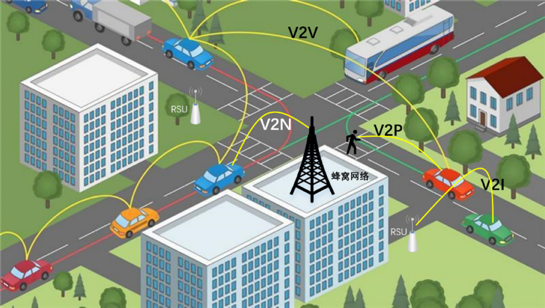
\includegraphics[width=0.35\textwidth]{fig/v2x.pdf}
  		\end{textblock*}
	\end{figure}
  \end{center}
  
\begin{center}
\begin{textblock*}{\textwidth}(-4cm,5cm)
\animategraphics[width=0.28\textwidth,autoplay,loop]{10}{fig/v2x3/v2x3-}{0}{20}\\\footnotesize 计算卸载与优化\\
\scriptsize 复杂任务 \hspace{1em} 多样性应用
\end{textblock*}
\end{center}

\begin{center}
\begin{textblock*}{\textwidth}(6cm,5cm)
\animategraphics[width=0.28\textwidth,autoplay,loop]{12}{fig/v2x4/v2x4-}{0}{24}\\ \footnotesize 智能交通系统\\
\scriptsize 碰撞预警 \hspace{1em} 自动驾驶
\end{textblock*}
\end{center}
\end{frame}

\begin{frame}{国家战略}
\frametitle{\englishfont 国家战略}
\newBackground
\begin{center}
\begin{textblock*}{\textwidth}(0.2cm,1.6cm)
\begin{figure}
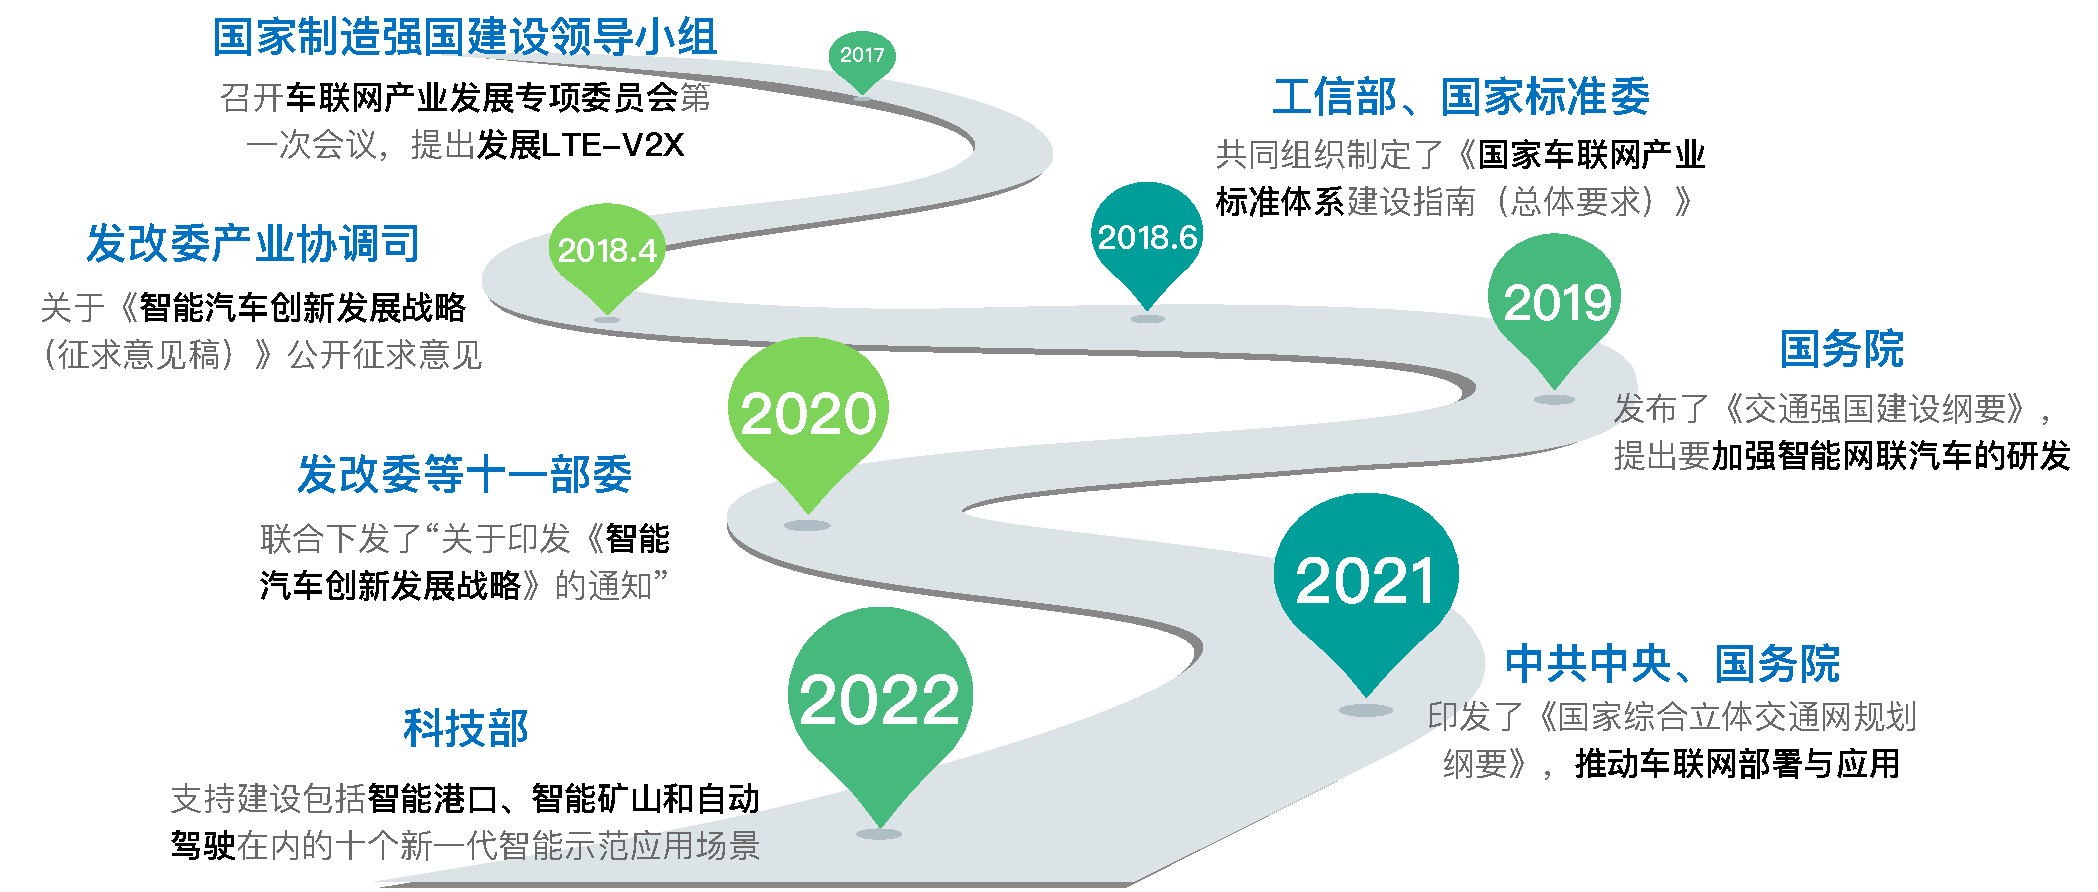
\includegraphics[width=1.1\textwidth]{fig/policy.pdf}
\end{figure}
\end{textblock*}
\end{center}
\end{frame}

\begin{frame}{V2X车联网}
\frametitle{\englishfont V2X车联网}
\newBackground
\begin{center}
\begin{textblock*}{\textwidth}(0.5cm,1.8cm)
\begin{figure}
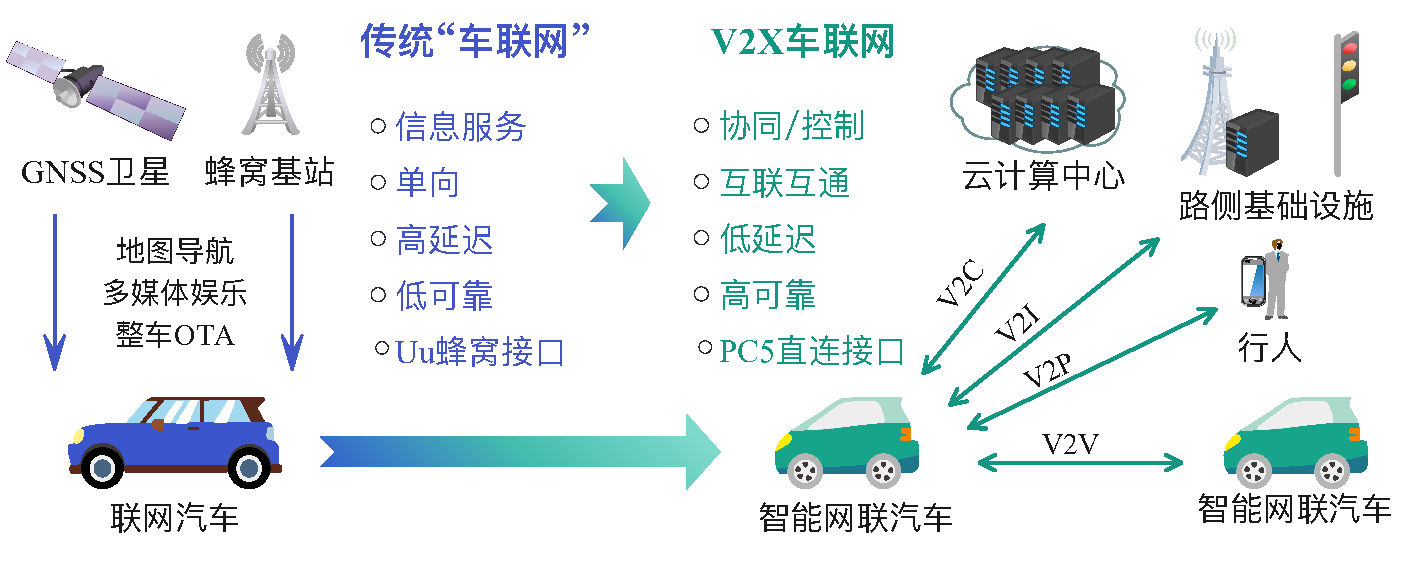
\includegraphics[width=1.1\textwidth]{fig/v2x-evolution.pdf}
\end{figure}
\end{textblock*}
\end{center}
\end{frame}

\subsection[\englishfont 1.2 车载信息物理融合系统]{1.2 车载信息物理融合系统}
\begin{frame}{车载信息物理融合系统}
\frametitle{\englishfont 车载信息物理融合系统 (Vehicular Cyber-Physical Systems, VCPS)}
\newBackground
\begin{center}
\begin{textblock*}{\textwidth}(1cm,1.8cm)
\begin{itemize} \englishfont
	\item[\ding{111}] {\color{cqublue}{关键思想}}
	\begin{itemize}
	\begin{footnotesize}
		\item[\ding{226}] 集成{\color{cqublue}{感知、计算、通信与控制}}技术
		\item[\ding{226}] 构建{\color{cqublue}{物理}}世界与{\color{cqublue}{虚拟}}世界的相互{\color{cqublue}{映射}}
	\end{footnotesize}
	\end{itemize}
	\item[\ding{111}]  {\color{cqublue}{发展历程}}
	\begin{itemize}
	\begin{footnotesize}
		\item[\ding{226}] 2006年,美国NSF启动CPS研究计划
		\item[\ding{226}] 2011年,LI等人首次将CPS引入车联网
	\end{footnotesize}
	\end{itemize}
\end{itemize}
\end{textblock*}
\end{center}

\begin{center}
\begin{textblock*}{\textwidth}(-2cm,5.2cm)
\begin{figure}
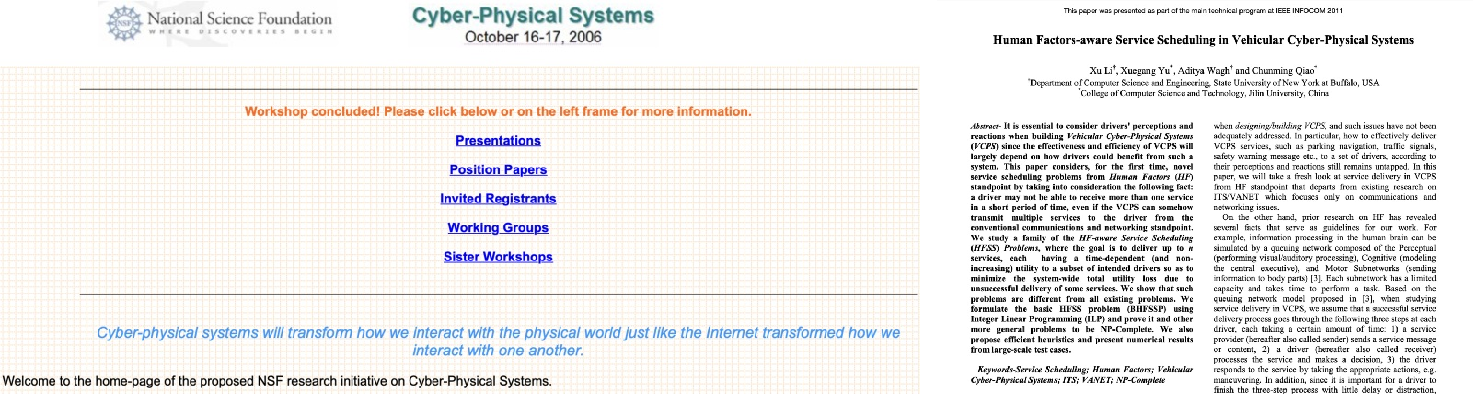
\includegraphics[width=0.6\textwidth]{fig/vcps_nsf.pdf}
\end{figure}
\end{textblock*}
\end{center}

\begin{center}
\begin{textblock*}{\textwidth}(5.5cm,1.8cm)
\begin{figure}
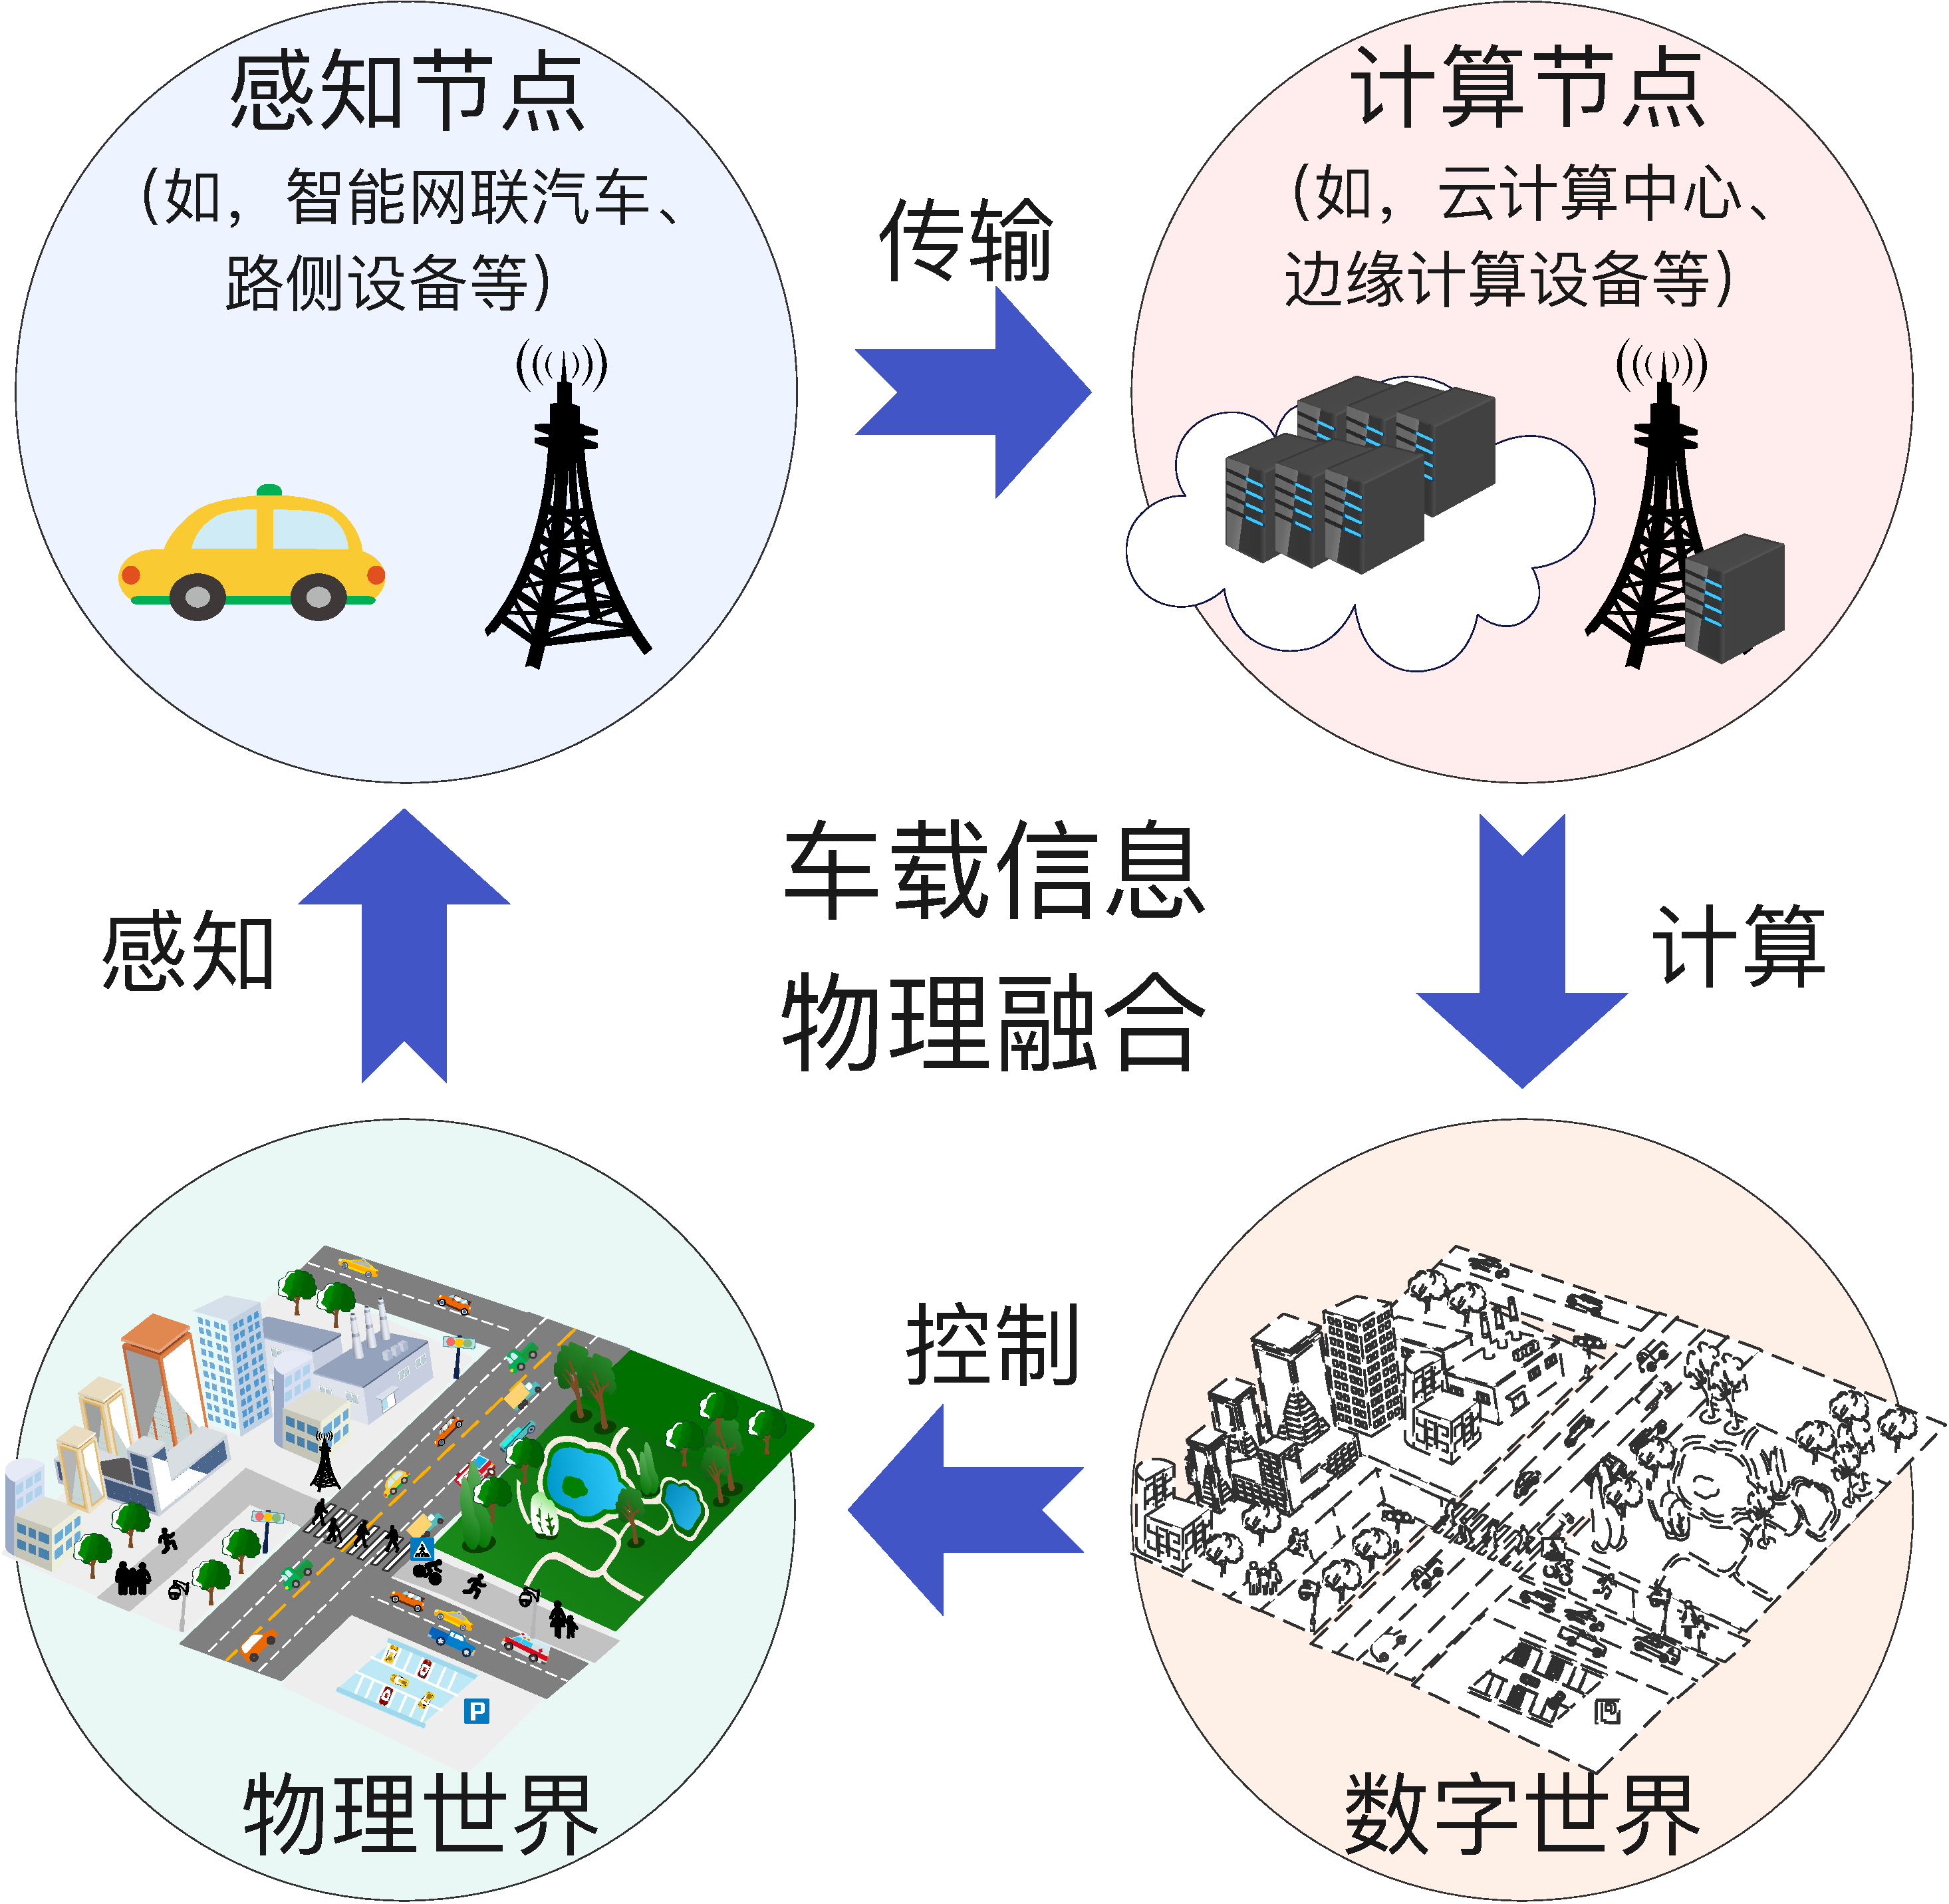
\includegraphics[width=0.45\textwidth]{fig/vcps.pdf}
\end{figure}
\end{textblock*}
\end{center}
\end{frame}

\begin{frame}{问题与挑战}
\frametitle{\englishfont 问题与挑战}
\newBackground
\begin{center}
\begin{textblock*}{\textwidth}(1cm,1.65cm)
\begin{figure}
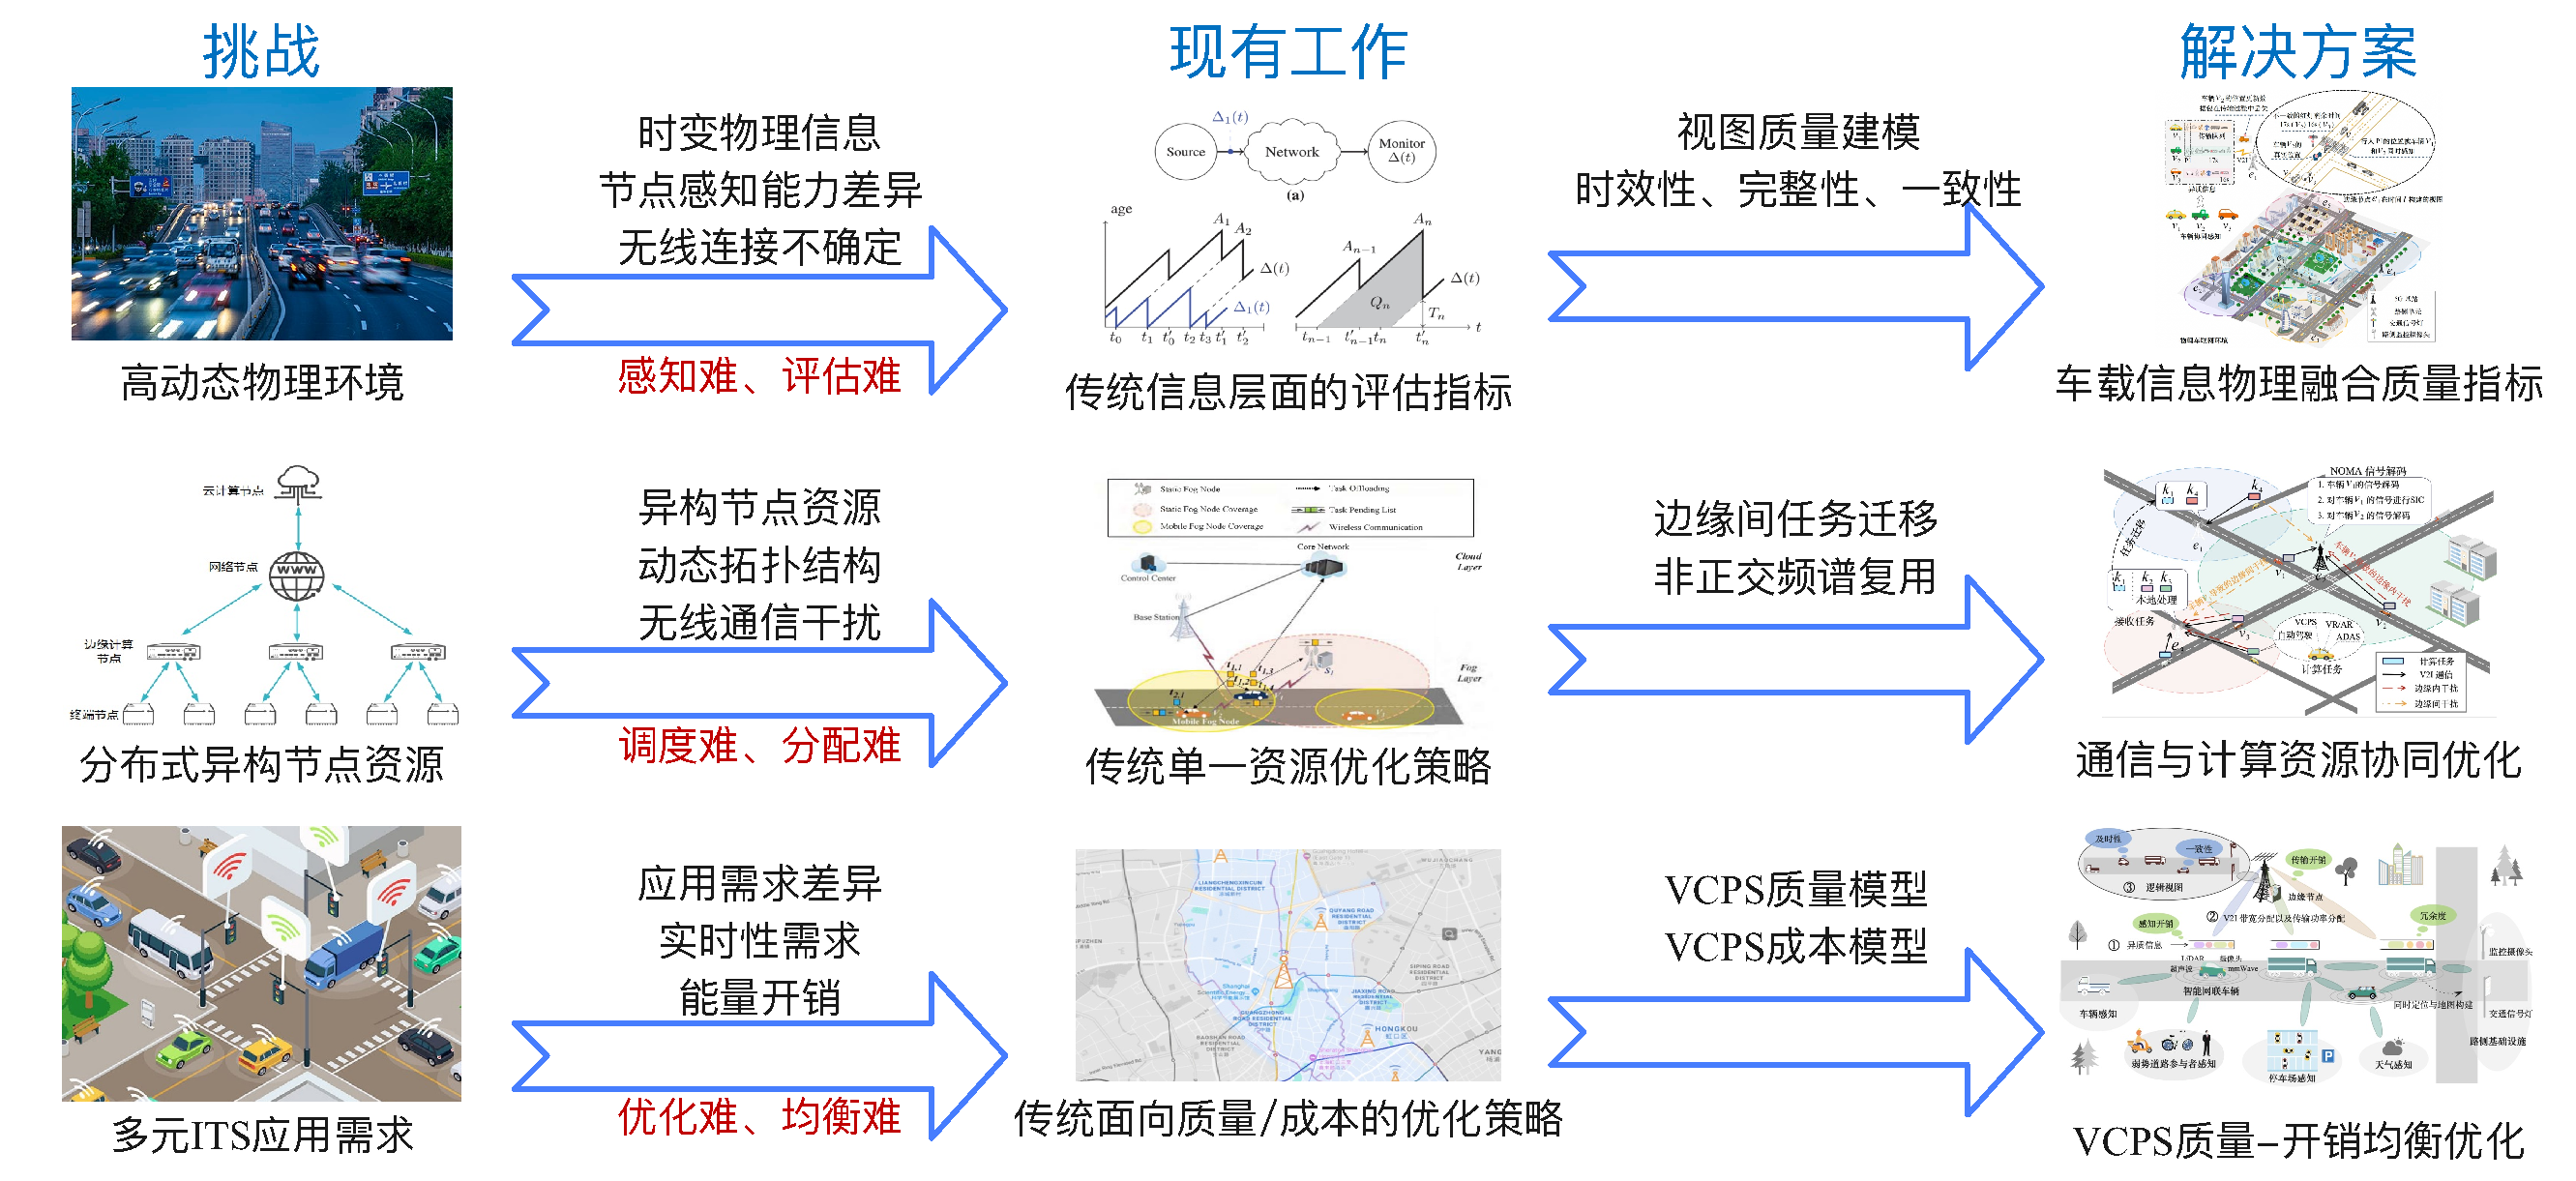
\includegraphics[width=1\textwidth]{fig/challenges.pdf}
\end{figure}
\end{textblock*}
\end{center}
\end{frame}


\begin{frame}{主要研究内容}
\frametitle{\englishfont 主要研究内容}
\newBackground
\begin{center}
\begin{textblock*}{\textwidth}(1cm,1.65cm)
\begin{figure}
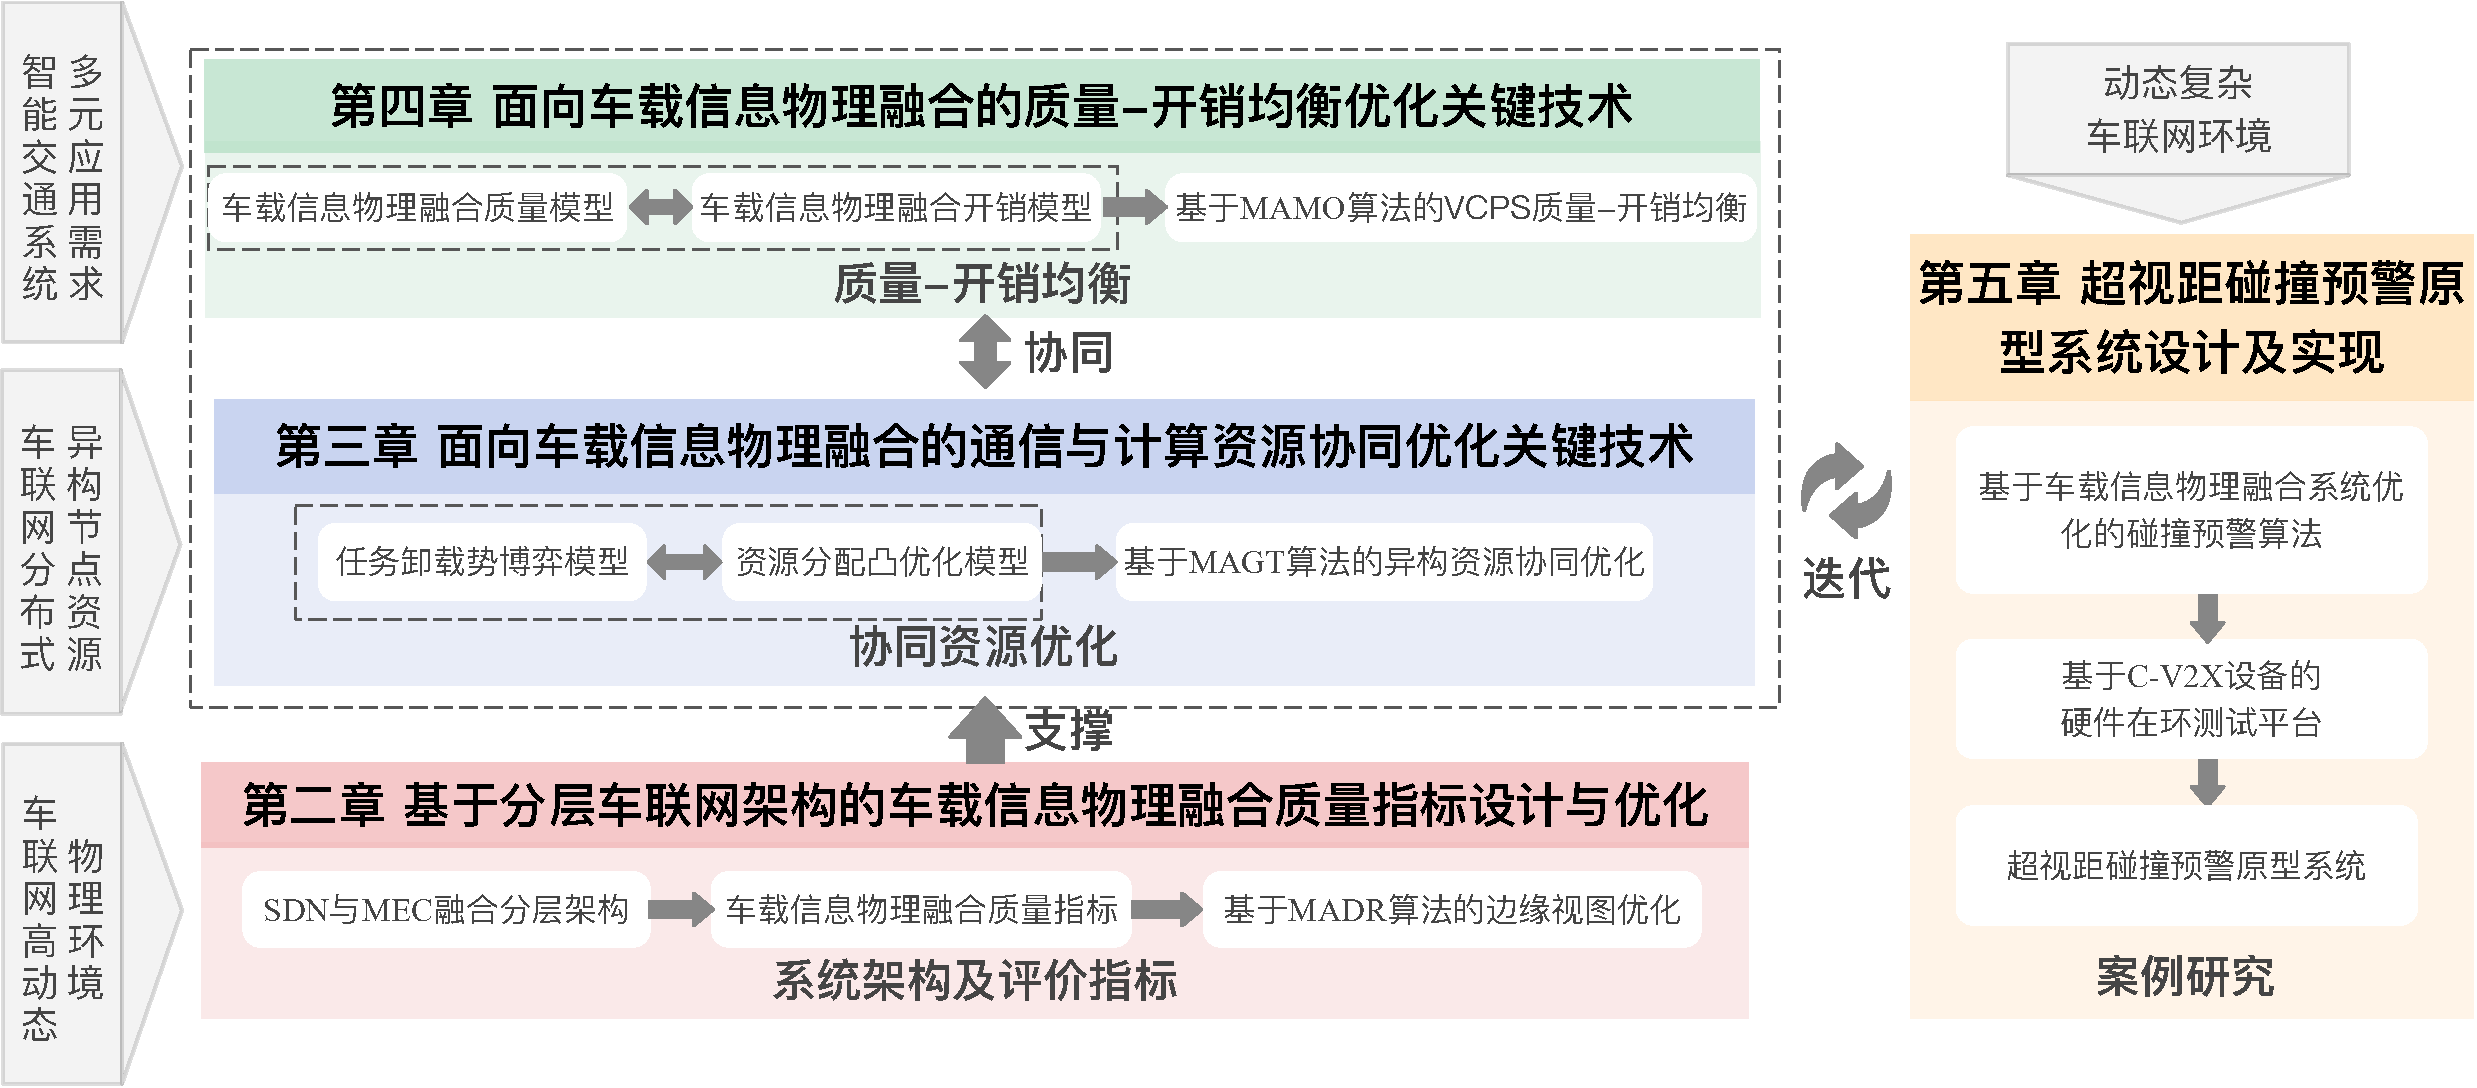
\includegraphics[width=1.05\textwidth]{fig/research_content.pdf}
\end{figure}
\end{textblock*}
\end{center}
\end{frame}